\documentclass{standalone}
\usepackage{tikz}
\usepackage{ctex,siunitx,ninecolors}
\setCJKmainfont{Noto Serif CJK SC}
\usepackage{tkz-euclide}
\usepackage{amsmath}
\usepackage{wasysym}
\usetikzlibrary{patterns, calc}
\usetikzlibrary{decorations.pathmorphing, decorations.pathreplacing, decorations.shapes,3d,backgrounds}
\newcommand{\hand}[2][0]{
  \begin{scope}[#2,rotate=#1,on background layer]
    \fill[pink!10!orange!10,draw=black,very thin]
    (-0.812, 0.563)..controls(-0.430, 0.531)and(-0.584, 0.282)..(-0.179, 0.197)..controls( 0.040, 0.131)and( 0.113, 0.007)..( 0.141,-0.072)--( 0.916,-0.020)..controls( 0.915, 0.319)and( 0.727, 0.379)..( 0.640, 0.609)..controls( 0.541, 0.843)and( 0.383, 0.790)..( 0.209, 0.818)..controls(-0.074, 0.877)and(-0.176, 0.901)..(-0.408, 1.006);
  \draw[very thin]
(0.122, 0.128)..controls(0.235, 0.126)and(0.288, 0.186)..(0.542, 0.499)
(0.459, 0.245)..controls(0.460, 0.199)and(0.559, 0.216)..(0.625, 0.410);
  \end{scope}
  \begin{scope}[#2,rotate=#1]
    \fill[pink!10!orange!10,draw=black,very thin]
    (-0.181, 0.373)..controls(-0.099, 0.290)and(-0.074, 0.245)..(-0.020, 0.228)..controls( 0.056, 0.195)and( 0.200, 0.208)..( 0.287, 0.139)..controls( 0.388, 0.065)and( 0.452,-0.156)..( 0.534,-0.196)..controls( 0.648,-0.315)and( 0.893,-0.305)..( 0.826,-0.169)..controls( 0.765,-0.009)and( 0.684, 0.104)..( 0.649, 0.152)..controls( 0.542, 0.285)and( 0.496, 0.354)..( 0.392, 0.463);
    \draw[very thin](0.772,-0.261)..controls(0.750,-0.255)and(0.726,-0.218)..
    (0.709,-0.192)..controls(0.677,-0.141)and(0.705,-0.102)..(0.758,-0.065)
    (0.595,-0.024)..controls(0.606,-0.008)and(0.640, 0.002)..(0.641, 0.022)
    (0.551, 0.047)..controls(0.596, 0.055)and(0.628, 0.092)..(0.632, 0.120);
  \end{scope}
}
\begin{document}
\small
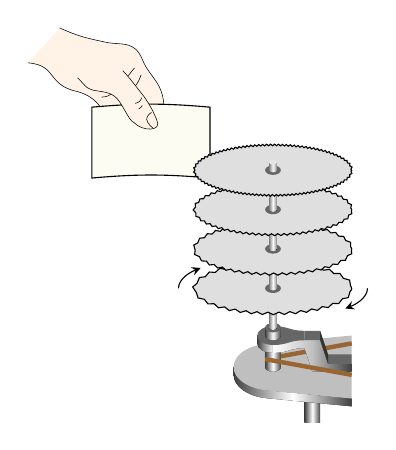
\begin{tikzpicture}[>=stealth]
  %%% 纸
  \draw[fill=yellow9!10!white](-2.3,2.3)to[bend left=5](-0.8,2.3)--(-0.8,1.4)to[bend right=5](-2.3,1.4)--cycle;
  %%% 机床
  \fill[left color=darkgray,right color=darkgray,middle color=white](0.4,-1.7)rectangle(0.6,-1.0);
  \fill[left color=darkgray,right color=darkgray,middle color=white]
  (-0.5,-1.1)arc(180:261:0.5 and 0.3)--(1,-1.5)--(1,-1.4)--(-0.0791,-1.2962)arc(261:180:0.5 and 0.3)--(-0.5,-1)--cycle;
  \fill[lightgray](1,-0.6)--(-0.0791,-0.7038)arc(99:261:0.5 and 0.3)--(1,-1.4);
  \draw[ultra thick,brown!80!black](-0.1,-0.9)--(1,-0.7);
  \fill[left color=darkgray,right color=darkgray,middle color=white](0,-1.0)ellipse(0.1 and 0.06);
  \fill[left color=darkgray,right color=darkgray,middle color=white](0.1,-0.6)rectangle(-0.1,-1.0);
  \fill[left color=darkgray,right color=darkgray,middle color=white](0,-0.7)ellipse(0.2 and 0.12);
  \fill[left color=darkgray,right color=darkgray,middle color=white](0.2,-0.6)rectangle(-0.2,-0.7);
  \fill[left color=white,right color=darkgray,middle color=lightgray](0,-0.82)..controls(0.2,-0.82)and(0.2,-0.76)..(0.4,-0.76)--(0.5,-1.06)--(1.0,-1.06)--(1.0,-0.96)--(0.7,-0.96)--(0.6,-0.66)--(0.4,-0.64)..controls(0.2,-0.64)and(0.2,-0.58)..(0,-0.58);
  \fill[darkgray!80](0,-0.72)..controls(0.2,-0.72)and(0.2,-0.66)..(0.4,-0.66)--(0.4,-0.54)..controls(0.2,-0.54)and(0.2,-0.48)..(0,-0.48);
  \fill[darkgray!80](0.4,-0.66)rectangle(0.6,-0.54)(0.7,-0.96)rectangle(1.0,-0.84);
  \fill[darkgray!80!black](0.6,-0.66)--(0.6,-0.54)--(0.7,-0.84)--(.7,-0.96);
  \fill[darkgray!80](0,-0.6)ellipse(0.2 and 0.12);
  \fill[left color=darkgray,right color=darkgray,middle color=white](0,-0.6)ellipse(0.1 and 0.06);
  \fill[left color=darkgray,right color=darkgray,middle color=white](0.1,-0.5)rectangle(-0.1,-0.6);
  \fill[darkgray!80](0,-0.5)ellipse(0.1 and 0.06);
  \fill[left color=gray,right color=gray,middle color=white](0,-0.5)ellipse(0.05 and 0.03);
  \fill[left color=gray,right color=gray,middle color=white](-0.05,-0.5)rectangle(0.05,0);
  \draw[ultra thick,brown!80!black](-0.1,-0.9)--(1,-1.1);
  %%% 齿轮
  \draw[decorate,decoration={zigzag,segment length=1.4mm,amplitude=0.16mm},fill=lightgray!50](0,0) ellipse (1 and 0.32);
  \fill[darkgray!80](0,0)ellipse(0.1 and 0.06);
  \fill[left color=gray,right color=gray,middle color=white](0,0)ellipse(0.05 and 0.03);
  \fill[left color=gray,right color=gray,middle color=white](-0.05,0)rectangle++(0.1,0.5);
  \draw[decorate,decoration={zigzag,segment length=1.1mm,amplitude=0.14mm},fill=lightgray!50](0,0.5) ellipse (1 and 0.32);
  \fill[darkgray!80](0,0.5)ellipse(0.1 and 0.06);
  \fill[left color=gray,right color=gray,middle color=white](0,0.5)ellipse(0.05 and 0.03);
  \fill[left color=gray,right color=gray,middle color=white](-0.05,0.5)rectangle++(0.1,0.5);
  \draw[decorate,decoration={zigzag,segment length=0.8mm,amplitude=0.12mm},fill=lightgray!50](0,1) ellipse (1 and 0.32);
  \fill[darkgray!80](0,1.0)ellipse(0.1 and 0.06);
  \fill[left color=gray,right color=gray,middle color=white](0,1.0)ellipse(0.05 and 0.03);
  \fill[left color=gray,right color=gray,middle color=white](-0.05,1.0)rectangle++(0.1,0.5);
  \draw[decorate,decoration={zigzag,segment length=0.5mm,amplitude=0.1mm}, fill=lightgray!50](0,1.5) ellipse (1 and 0.32);
  \fill[darkgray!80](0,1.5)ellipse(0.1 and 0.06);
  \fill[left color=gray,right color=gray,middle color=white](0,1.5)ellipse(0.05 and 0.03);
  \fill[left color=gray,right color=gray,middle color=white](-0.05,1.5)rectangle++(0.1,0.1);
  \fill[gray!20](0,1.6)ellipse(0.05 and 0.03);
  \draw[thin,->](1.2,0)arc(0:-40:1.2 and 0.4);
  \draw[thin,->](-1.2,0)arc(180:140:1.2 and 0.4);
  \hand{xshift=-2.3cm,yshift=2.3cm}
\end{tikzpicture}
\end{document}